\chapter{Application of optimization algorithms}

In this chapter, we describe the problem-specific details of our chosen optimization algorithms. Section~\ref{sec:initial_schedules} presents different options for creating initial schedules and explains which ones were chosen for optimization. Section~\ref{sec:coding_of_a_solution} describes the format of non-trivial schedules that we optimize. Sections~\ref{sec:genetic_algorithm_application},~\ref{sec:hill_climbing_application}, and~\ref{sec:simulated_annealing_application} cover the exact configuration of genetic algorithm, hill climbing, and simulated annealing, respectively, including their hyperparameters. Section~\ref{sec:hyperparameter_search} explains how we searched for the best hyperparameters and summarizes the final settings for each algorithm and dataset.

\section{Initial schedules} \label{sec:initial_schedules}

The creation of initial schedules is part of the simulator's functionality and makes use of \hyperref[para:heuristic_1]{Heuristic 1}.
Each schedule of an intersection consists of two parts: \textit{order} and \textit{times}. Order is an array of street indices that defines the order in which the streets have the green light. Times is an array of integers that defines the duration of the green light with respect to the street order. To keep the two parts consistent, \textit{any changes to the order array must also be applied to the corresponding times array}.

We provide a few different initialization options for both order and times. Order initializations include:
\begin{itemize}
    \item \textit{default} - simply uses the order given by street IDs in the input file
    \item \textit{random} - takes a random permutation of the streets
    \item \textit{adaptive} - determines the order during a simulation run; whenever a street is used for the first time, it is assigned to the earliest free position in the order array (only usable with the \textit{default} times initialization)
\end{itemize}
Times initializations include:
\begin{itemize}
    \item \textit{default} - all times are set to 1 second
    \item \textit{scaled} - time for each street is a total number of cars using this street divided by a single given constant (the divisor)
\end{itemize}
Default order and default times represent our \textit{baseline} solution.

Both \texttt{order initialization} and \texttt{times initialization} are hyperparameters. To decide which setting to use for optimization, we experimentally compared scores of different initialization options across all datasets.

The results are shown in Figure~\ref{fig:init_comparison}. We can see that by using other ``smarter'' initialization methods, we can significantly improve the baseline solution and start optimizing from much better starting points.
We decided to use \textit{adaptive order} and \textit{default times} for datasets B, C, and D, and \textit{random order} and \textit{scaled times} for datasets E and F (see Table~\ref{tab:hyperparams_datasets_specific}).

\begin{figure}[h]
    \centering
    % 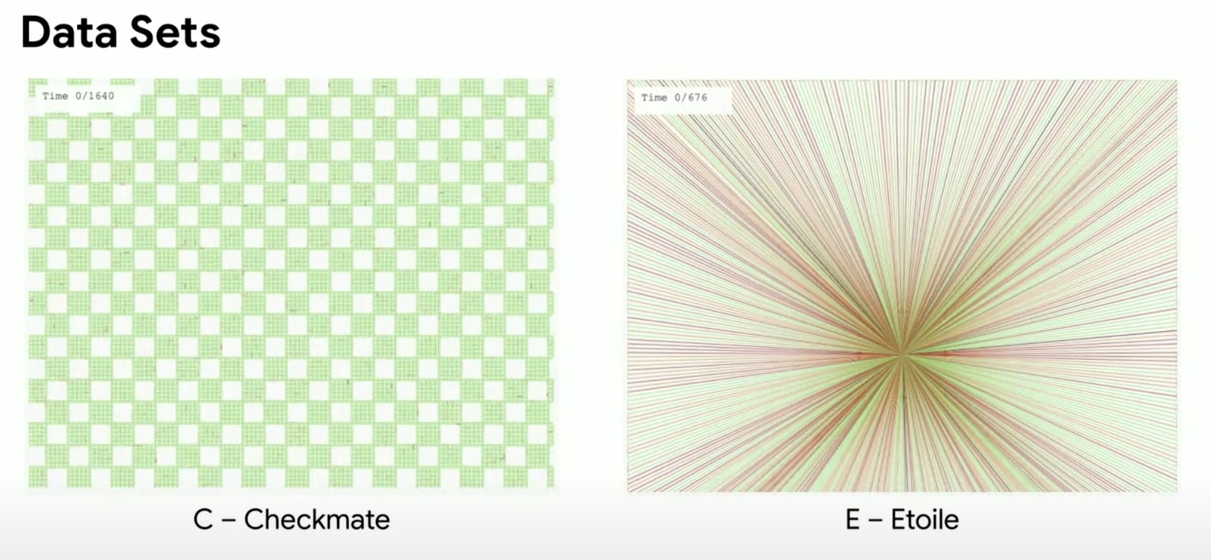
\includegraphics[width=.8\linewidth]{img/screenshots/hashcode_datasets_c_e.png}
    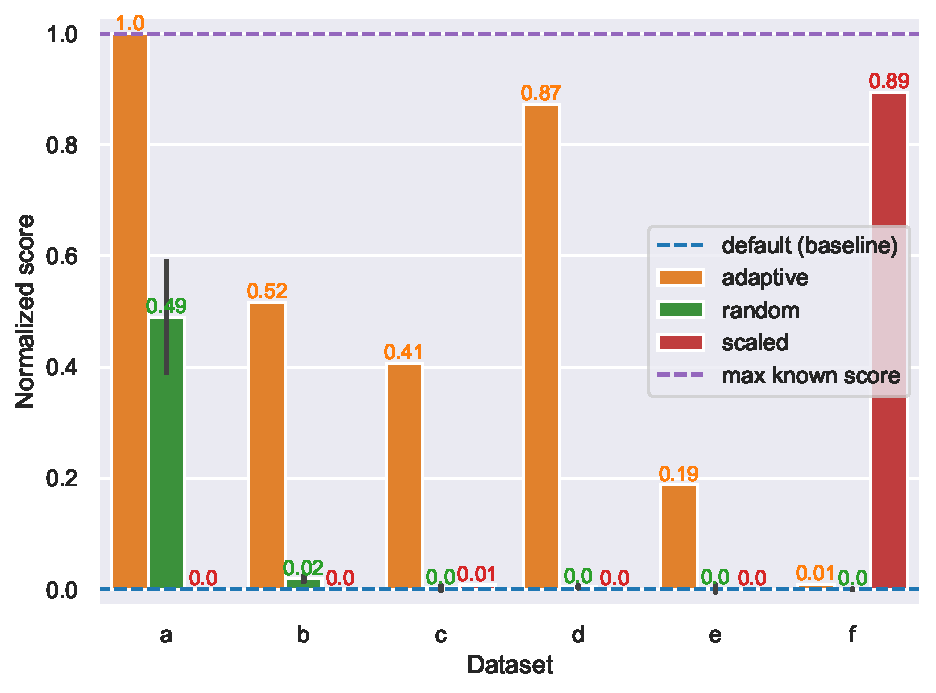
\includegraphics[width=\linewidth]{img/experiments/init_experiment.pdf}
    \caption[Comparison of initialization options]{
        Comparison of different initialization options across datasets.
        Specifically, we compare \textcolor{myorange}{\textbf{adaptive}} (adaptive order and default times), \textcolor{mygreen}{\textbf{random}} (random order and default times), and \textcolor{myred}{\textbf{scaled}} (default order and scaled times) options. \textcolor{myblue}{\textbf{Default}} (default order and default times) option represents the baseline solution.
        \textcolor{mygreen}{\textbf{Random}} option is averaged over 100 trials, the black error bars show the 95\% confidence interval.
        For \textcolor{myred}{\textbf{scaled}} option, we use the best divisor between 1--100 for each dataset.
        Y-axis shows the normalized score, where 0 is the baseline score and 1 is the maximum known score for each dataset.
    }
    \label{fig:init_comparison}
\end{figure}

\section{Coding of non-trivial schedules} \label{sec:coding_of_a_solution}

As explained in Section~\ref{sec:further_insights_and_heuristics}, specifically in \hyperref[para:heuristic_2]{Heuristic 2}, we only optimize the non-trivial schedules. The simulator returns the non-trivial schedules in the following format:
\begin{quote}
    a \textbf{list of pairs}, where each pair consists of \textbf{order} and \textbf{times} arrays.
\end{quote}
Analogously, the simulator accepts the non-trivial schedules in the same format when updating them for evaluation.

This is the format---the encoding of a state or solution, if you will---that we use for all of the optimization algorithms. In this setup, we simply treat the non-trivial schedules as states within a black-box optimization.
Since the state structure is quite complex, and each intersection's schedule can have a different number of streets, any modifications are applied separately for each intersection.

\section{Genetic algorithm} \label{sec:genetic_algorithm_application}

In this section, we apply the theory introduced in Section~\ref{sec:genetic_algorithm} and describe our design of the genetic algorithm, including the selection, crossover, and mutation operators, as well as the corresponding hyperparameters. We begin with this method, as the other algorithms reuse its mutation operator to generate new states.

\subsection{Selection}

For selecting individuals for reproduction, we use \textit{tournament selection} combined with \textit{elitism}. The corresponding hyperparameters are \texttt{tournament size} and \texttt{elitism}, which defines the percentage of top-performing individuals that are directly selected for reproduction.
\subsection{Crossover}

For each intersection, we randomly decide whether to crossover only the order, only the times, or both. We use \textit{order crossover (OX)} for modifying the order, and \textit{two-point crossover} for modifying the times. Crossover is performed with a probability defined by the hyperparameter \texttt{crossover probability}.

\subsection{Mutation} \label{sec:mutation_application}

For each intersection, we randomly decide whether to mutate only the order, only the times, or both. We use \textit{index shuffle} for modifying the order, and for the times, we add or subtract one to some values at random. Mutation is performed with a probability defined by the hyperparameter \texttt{mutation probability}. When mutation is applied, the hyperparameter \texttt{mutation bit rate} controls how likely each individual value is to be modified. It can be given either as a probability or as an integer specifying the expected number of modified values in the state.

\bigskip

The remaining hyperparameters of the genetic algorithm are \texttt{population size} and \texttt{generations}---their names are quite self-explanatory. Together with the crossover and mutation probabilities, these hyperparameters control the total number of fitness evaluations (i.e., simulation runs) performed by the algorithm.

\section{Hill climbing} \label{sec:hill_climbing_application}

As explained in Section~\ref{sec:hill_climbing}, we use a variant of the algorithm that generates next states randomly because there is no explicit neighborhood structure. We simply apply the mutation operator from the genetic algorithm (see Section~\ref{sec:mutation_application}) to generate the next state. Note that we again use the hyperparameter \texttt{mutation bit rate} but not the mutation probability because the mutation is always applied. The only other hyperparameter is \texttt{iterations}, which sets the number of iterations the algorithm runs for.

\section{Simulated annealing} \label{sec:simulated_annealing_application}

Introduced in Section~\ref{sec:simulated_annealing}, this algorithm uses the same startegy to generate next states as presented in Section~\ref{sec:hill_climbing_application}. That means it has the same hyperaparameters \texttt{mutation bit rate} and \texttt{iterations}. The only additional hyperparameter is \texttt{initial temperature}, which sets the initial temperature of the cooling schedule. For the cooling schedule, we use a linear decay. It is defined as
\begin{equation}
    schedule(t) = \tau_{init} \cdot \left(1 - \frac{t}{T}\right) + \varepsilon,
\end{equation}
where $\tau_{init}$ is the \texttt{initial temperature}, $t$ is the current iteration, and $T$ is the total number of \texttt{iterations}.
% Both of these values are hyperparameters, with the initial temperature especially requiring careful tuning for each dataset to achieve good results.

\section{Hyperparameter search} \label{sec:hyperparameter_search}

Performance of all three aforementioned algorithms largely depends on the setting of their hyperparameters.
To find the best hyperparameters for the experiments, we use a form of \textit{greedy search}. That is, we only focus on optimizing one hyperparameter at a time and try to find the best value for it. Other hyperparameters are currently fixed---either heuristically or set to their already optimized values.
We test a number of reasonable values for each hyperparameter and perform runs with additional values if the results are not satisfactory.
Each setting is tested on 10 different fixed seeds and the results are averaged.

To maintain comparability, we allocate an equal budget of fitness evaluations to all three algorithms. For hill climbing and simulated annealing, this budget is easily enforced via the \texttt{iterations} hyperparameter. For genetic algorithm, the number of evaluations is stochastic and cannot be precisely set; however, we always set the \texttt{generations} hyperparameter so that the expected total number of fitness evaluations matches the predefined budget.

For each dataset, we use the best initialization options that we selected in Section~\ref{sec:initial_schedules}.

% TABLE WITH TESTED HYPERPARAMETER VALUES
\begin{table}[h]
\centering\footnotesize\sf

\begin{tabular}{l@{\hspace{0.5cm}}c}
% \toprule
% \multicolumn{2}{l}{\textbf{Tested values}} \\
Crossover probability & $[0.2, 0.3, \cdots 0.8]$ \\
Mutation probability & $[0.1, 0.2, \cdots 1.0]$ \\
Tournament size & $[2, 3, \cdots, 10]$ \\
Elitism & $[0, 0.05, 0.1, \cdots, 0.3]$ \\
Population size & $[10, 20, \cdots, 100]$ \\
% \midrule
Mutation bit rate & $[1, 2, \cdots, 20]$ \\
Initial temperature & many values between $0.1$ and $500$ \\
% \bottomrule
\end{tabular}

\caption[Tested hyperparameter values]{Ranges of tested hyperparameter values.}
\label{tab:hyperparams_tested_values}
\end{table}

To give a clearer picture of the values explored, Table~\ref{tab:hyperparams_tested_values} summarizes the ranges used in the hyperparameter search. 
The genetic algorithm parameters---\texttt{crossover probability}, \texttt{mutation probability}, \texttt{tournament size}, and \texttt{elitism}---were tested only on smaller datasets E and B to reduce search complexity, because they seemed generalizable across datasets. Other parameters, especially the \texttt{mutation bit rate} and \texttt{initial temperature}, are highly dataset-dependent and were tuned separately for each algorithm and dataset.

\newpage

Finally, Tables~\ref{tab:hyperparams_shared} and~\ref{tab:hyperparams_datasets_specific} provide a detailed overview of the selected hyperparameters for the experiments. For clarity, the first table lists the hyperparameters that are shared across all datasets, while the second table shows dataset-specific hyperparameters.

% TABLE WITH SHARED HYPERPARAMETERS
\begin{table}[h]
\centering\footnotesize\sf

\begin{tabular}{l@{}c}
% \toprule
\multicolumn{2}{l}{\textbf{Genetic Algorithm}} \\
Crossover probability & 0.6 \\
Mutation probability & 0.4 \\
Tournament size & 3 \\
Elitism & 0.05 \\
\midrule
\multicolumn{2}{l}{\textbf{Hill Climbing}} \\
Iterations & 450000 \\
\midrule
\multicolumn{2}{l}{\textbf{Simulated Annealing}} \\
Iterations & 450000 \\
% \bottomrule
\end{tabular}

\caption[Shared hyperparameters]{Shared hyperparameters for all datasets.}
\label{tab:hyperparams_shared}
\end{table}

% TABLE WITH DATASET-SPECIFIC HYPERPARAMETERS
\begin{table}[h]
\centering\footnotesize\sf

\begin{minipage}[t]{0.48\textwidth}
\centering
\begin{tabular}{l@{\hspace{0.5cm}}c}
% \toprule
\multicolumn{2}{c}{\textbf{Dataset E}} \\
\midrule
Order initialization & random \\
Times initialization & scaled \\
\midrule
\multicolumn{2}{l}{\textbf{Genetic Algorithm}} \\
Population size & 90 \\
Generations & 6667 \\
Mutation bit rate & 9 \\
\midrule
\multicolumn{2}{l}{\textbf{Hill Climbing}} \\
Mutation bit rate & 15 \\
\midrule
\multicolumn{2}{l}{\textbf{Simulated Annealing}} \\
Mutation bit rate & 5 \\
Initial temperature & 275 \\
% \bottomrule
\end{tabular}
\end{minipage}
\hfill
\begin{minipage}[t]{0.48\textwidth}
\centering
\begin{tabular}{l@{\hspace{0.5cm}}c}
% \toprule
\multicolumn{2}{c}{\textbf{Dataset B}} \\
\midrule
Order initialization & adaptive \\
Times initialization & default \\
\midrule
\multicolumn{2}{l}{\textbf{Genetic Algorithm}} \\
Population size & 10 \\
Generations & 60000 \\
Mutation bit rate & 2 \\
\midrule
\multicolumn{2}{l}{\textbf{Hill Climbing}} \\
Mutation bit rate & 4 \\
\midrule
\multicolumn{2}{l}{\textbf{Simulated Annealing}} \\
Mutation bit rate & 1 \\
Initial temperature & 0.25 \\
% \bottomrule
\end{tabular}
\end{minipage}
\newline
\newline
\newline
\begin{minipage}[t]{0.48\textwidth}
\centering
\begin{tabular}{l@{\hspace{0.5cm}}c}
% \toprule
\multicolumn{2}{c}{\textbf{Dataset F}} \\
\midrule
Order initialization & random \\
Times initialization & scaled \\
\midrule
\multicolumn{2}{l}{\textbf{Genetic Algorithm}} \\
Population size & 50 \\
Generations & 12000 \\
Mutation bit rate & 2 \\
\midrule
\multicolumn{2}{l}{\textbf{Hill Climbing}} \\
Mutation bit rate & 5 \\
\midrule
\multicolumn{2}{l}{\textbf{Simulated Annealing}} \\
Mutation bit rate & 3 \\
Initial temperature & 15 \\
% \bottomrule
\end{tabular}
\end{minipage}
\hfill
\begin{minipage}[t]{0.48\textwidth}
\centering
\begin{tabular}{l@{\hspace{0.5cm}}c}
% \toprule
\multicolumn{2}{c}{\textbf{Dataset C}} \\
\midrule
Order initialization & adaptive \\
Times initialization & default \\
\midrule
\multicolumn{2}{l}{\textbf{Genetic Algorithm}} \\
Population size & 20 \\
Generations & 30000 \\
Mutation bit rate & 2 \\
\midrule
\multicolumn{2}{l}{\textbf{Hill Climbing}} \\
Mutation bit rate & 4 \\
\midrule
\multicolumn{2}{l}{\textbf{Simulated Annealing}} \\
Mutation bit rate & 2 \\
Initial temperature & 0.1 \\
% \bottomrule
\end{tabular}
\end{minipage}
\newline
\newline
\newline
\begin{minipage}[t]{0.48\textwidth}
\centering
\begin{tabular}{l@{\hspace{0.5cm}}c}
% \toprule
\multicolumn{2}{c}{\textbf{Dataset D}} \\
\midrule
Order initialization & adaptive \\
Times initialization & default \\
\midrule
\multicolumn{2}{l}{\textbf{Genetic Algorithm}} \\
Population size & 40 \\
Generations & 15000 \\
Mutation bit rate & 2 \\
\midrule
\multicolumn{2}{l}{\textbf{Hill Climbing}} \\
Mutation bit rate & 2 \\
\midrule
\multicolumn{2}{l}{\textbf{Simulated Annealing}} \\
Mutation bit rate & 2 \\
Initial temperature & 0.1 \\
% \bottomrule
\end{tabular}
\end{minipage}

\caption[Dataset-specific hyperparameters]{
    Dataset-specific hyperparameters.
    The order and times initializations are the same for all three methods for each dataset.
}
\label{tab:hyperparams_datasets_specific}
\end{table}
